\documentclass[11pt]{article}
% Change "article" to "report" to get rid of page number on title page
\usepackage{amsmath,amsfonts,amsthm,amssymb}

\usepackage{ulem}
\usepackage{framed}
\usepackage{setspace}
\usepackage{Tabbing}
\usepackage{fancyhdr}
\usepackage{lastpage}
\usepackage{extramarks}
\usepackage{chngpage}
\usepackage{soul,color}
\usepackage{graphicx,float,wrapfig}
\usepackage{relsize}
\usepackage{booktabs}
\usepackage{cellspace}
\usepackage{wrapfig}
\usepackage{lipsum}


\graphicspath{ {c:/user/images/} }
\usepackage[rightcaption]{sidecap}
\usepackage{blindtext}
\usepackage{hyperref}

\hypersetup{
    colorlinks=true,
    linkcolor=blue,
    filecolor=magenta,      
    urlcolor=cyan,
    pdftitle={Sharelatex Example},
    bookmarks=true,
    pdfpagemode=FullScreen,
    }
    
\urlstyle{same}

% In case you need to adjust margins:
\topmargin=-0.45in      %
\evensidemargin=0in     %
\oddsidemargin=0in      %
\textwidth=6.5in        %
\textheight=9.0in       %
\headsep=0.25in         %

% Homework Specific Information
\newcommand{\hmwkTitle}{How Does Climate Change Influence Regional Instability?}
\newcommand{\hmwkDueDate}{}
\newcommand{\hmwkClass}{Problem E}
\newcommand{\hmwkAuthorName}{Team 91611}

% Setup the header and footer
\pagestyle{fancy}                                                       %
\lhead{\hmwkAuthorName}                                                 %
\chead{\hmwkClass\ - \hmwkTitle}
  %
\rhead{}
  %
\lfoot{\lastxmark}                                                      %
\cfoot{}                                                                %
\rfoot{Page\ \thepage\ of\ \pageref{LastPage}}                          %
\renewcommand\headrulewidth{0.4pt}                                      %
\renewcommand\footrulewidth{0.4pt}                                      %
\newcommand{\enterProblemHeader}[1]{\nobreak\extramarks{#1}{#1 continued on next page\ldots}\nobreak%
                                    \nobreak\extramarks{#1 (continued)}{#1 continued on next page\ldots}\nobreak}%
\newcommand{\exitProblemHeader}[1]{\nobreak\extramarks{#1 (continued)}{#1 continued on next page\ldots}\nobreak%
                                   \nobreak\extramarks{#1}{}\nobreak}%

\newlength{\labelLength}
\newcommand{\labelAnswer}[2]
  {\settowidth{\labelLength}{#1}%
   \addtolength{\labelLength}{0.25in}%
   \changetext{}{-\labelLength}{}{}{}%
   \noindent\fbox{\begin{minipage}[c]{\columnwidth}#2\end{minipage}}%
   \marginpar{\fbox{#1}}%

   % We put the blank space above in order to make sure this
   % \marginpar gets correctly placed.
   \changetext{}{+\labelLength}{}{}{}}%

\setcounter{secnumdepth}{0}
\newcommand{\homeworkProblemName}{}%
\newcounter{homeworkProblemCounter}%
\newenvironment{homeworkProblem}[1][Problem \arabic{homeworkProblemCounter}]%
  {\stepcounter{homeworkProblemCounter}%
   \renewcommand{\homeworkProblemName}{#1}%
   \section{\homeworkProblemName}%
   \enterProblemHeader{\homeworkProblemName}}%
  {\exitProblemHeader{\homeworkProblemName}}%

\newcommand{\problemAnswer}[1]
  {\noindent\fbox{\begin{minipage}[c]{\columnwidth}#1\end{minipage}}}%

\newcommand{\problemLAnswer}[1]
  {\labelAnswer{\homeworkProblemName}{#1}}

\newcommand{\homeworkSectionName}{}%
\newlength{\homeworkSectionLabelLength}{}%
\newenvironment{homeworkSection}[1]%
  {% We put this space here to make sure we're not connected to the above.
   % Otherwise the changetext can do funny things to the other margin

   \renewcommand{\homeworkSectionName}{#1}%
   %\settowidth{\homeworkSectionLabelLength}{\homeworkSectionName}%
   %\addtolength{\homeworkSectionLabelLength}{0in}%
   \changetext{}{-\homeworkSectionLabelLength}{}{}{}%
   \subsection{\homeworkSectionName}%
   \enterProblemHeader{\homeworkProblemName\ [\homeworkSectionName]}}%
  {\enterProblemHeader{\homeworkProblemName}%

   % We put the blank space above in order to make sure this margin
   % change doesn't happen too soon (otherwise \sectionAnswer's can
   % get ugly about their \marginpar placement.
   \changetext{}{+\homeworkSectionLabelLength}{}{}{}}%

\newcommand{\sectionAnswer}[1]
  {% We put this space here to make sure we're disconnected from the previous
   % passage

   \noindent\fbox{\begin{minipage}[c]{\columnwidth}#1\end{minipage}}%
   \enterProblemHeader{\homeworkProblemName}\exitProblemHeader{\homeworkProblemName}%
   %\marginpar{\fbox{\homeworkSectionName}}%

   % We put the blank space above in order to make sure this
   % \marginpar gets correctly placed.
   }%

%%%%%%%%%%%%%%%%%%%%%%%%%%%%%%%%%%%%%%%%%%%%%%%%%%%%%%%%%%%%%


%%%%%%%%%%%%%%%%%%%%%%%%%%%%%%%%%%%%%%%%%%%%%%%%%%%%%%%%%%%%%
% Make title
\title{\vspace{2in}\textmd{\textbf{\hmwkClass:\ \hmwkTitle}}\\\normalsize\vspace{0.1in}\small{ \hmwkDueDate}\\\vspace{0.1in}\large{\textit{\hmwkClassInstructor\ \hmwkClassTime}}\vspace{3in}}
\date{}
\author{\textbf{\hmwkAuthorName}}
%%%%%%%%%%%%%%%%%%%%%%%%%%%%%%%%%%%%%%%%%%%%%%%%%%%%%%%%%%%%%
\begin{document}
\begin{spacing}{1.1}
\maketitle
\newpage
% Uncomment the \tableofcontents and \newpage lines to get a Contents page
% Uncomment the \setcounter line as well if you do NOT want subsections
%       listed in Contents
%\setcounter{tocdepth}{1}
\tableofcontents
\newpage

% When problems are long, it may be desirable to put a \newpage or a
% \clearpage before each homeworkProblem environment

\newpage
\begin{homeworkProblem}[Summary Sheet]
    Climate Change is rapidly increasing in today’s world. As it does, it affects how fragile the governments of countries around the world are becoming.  In order to attempt to begin to mitigate these affects, Climate Change’s impact on governmental fragility must be understood.
    \begin{homeworkSection}{Task 1}
        The model presented here utilizes three distinct components to track the fragility of a given country’s government. These components are as follows: Baseline Fragility, $F$; Climate Change, $C$; and Vulnerability, $V$. Baseline Fragility represents how fragile a country would be in a hypothetical world where Climate Change did not exist. The Climate Change component uses Global Temperature data to represent the intensity of Climate Change. Lastly, the Vulnerability component considers how susceptible a country is to effects of climate change.  All these components are combined, $F + (C\cdotV)$, and a score is produced.  The potential scores are split into thirds, the top third indicates a fragile state, the middle third a vulnerable state, and the bottom third a stable one.  The component of a country’s fragility that is dependent on Climate Change can be evaluated by considering its corresponding component, $(C\cdot V)$.
    \end{homeworkSection}
    \begin{homeworkSection}{Task 2}
        All the collected data regarding Chad's GDP growth and surface temperature fluctuations serves as fairly strong evidence that suggests that the effects of climate change played a vital role in the fragility of Chad.
    \end{homeworkSection}
    \begin{homeworkSection}{Task 3}
        This model was used to analyze the country Botswana. It falls geographically in a semi-arid region and is particularly susceptible to droughts and flooding which impacts many sectors that impact its fragility, for example its agricultural sector. This model predicts when it will cross a rough-estimate threshold to be a Fragile State from the critical zone.
    \end{homeworkSection}
    \begin{homeworkSection}{Task 4}
        Using pre-existing ideology and research about the specific distribution of resources to mitigate Climate Change Effects, along with the model to compute relative need of aid compared to all other countries listed, the proposed solution, in terms of millions of dollars, scales the distribution by the need of aid. Botswana is used as an example.
    \end{homeworkSection}
    \begin{homeworkSection}{Task 5}
        This model is not adaptable to be scaled up to a continent or down to a city. It is highly dependent on data that relates specifically to entire countries. In order to adapt this model to a larger or smaller scope new data regarding the area in question would need to be acquired.
    \end{homeworkSection}   
\end{homeworkProblem}
\newpage
\begin{homeworkProblem}[Pre-Amble]
    
    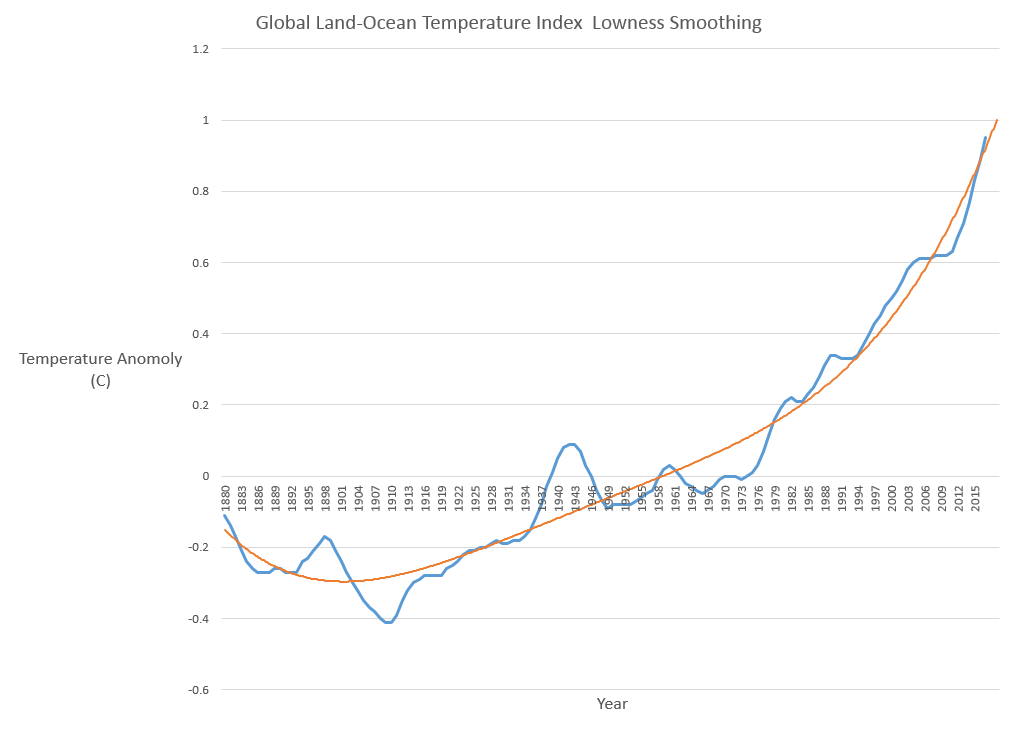
\includegraphics[angle=270, scale=0.8]{Global_Temperature}
    \newpage
    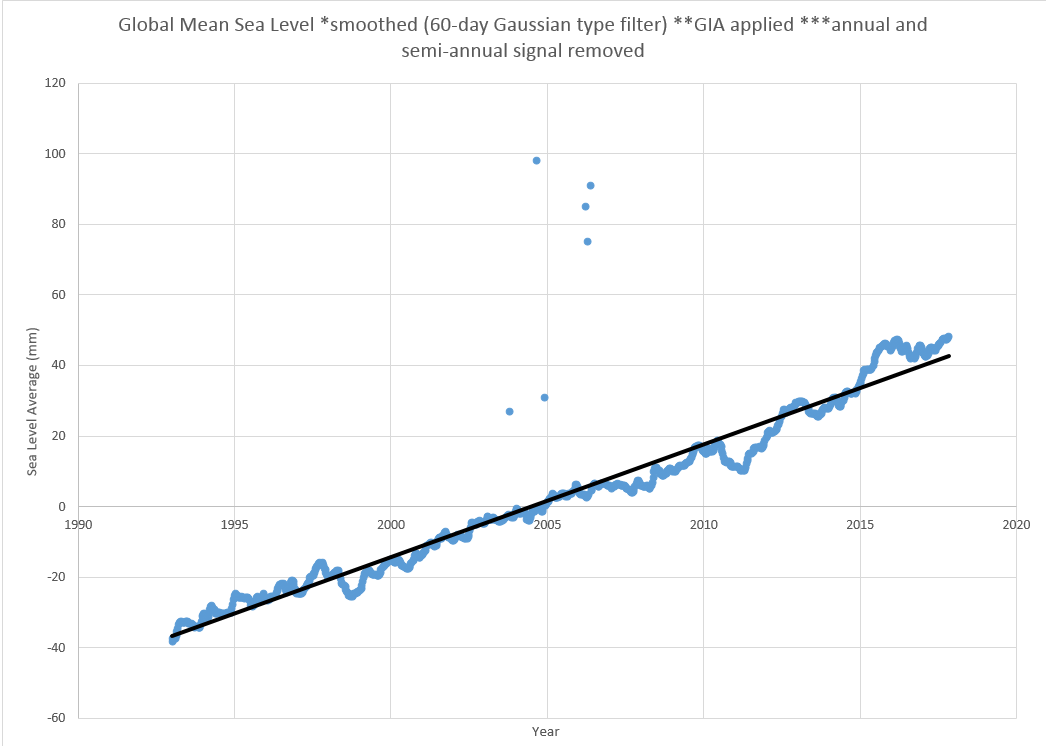
\includegraphics[angle=270, scale=0.8]{Water_Levels}
    \newpage
    \noindent
    Climate change is a serious threat for the upcoming decades. As it causes the changes shown in the graphs above and other drastic changes in the environment, it is bound to have serious adverse effects on human beings. One way to begin to look at these impacts on human behavior and organization is through the analysis of governmental structures throughout the world.  Some countries are in areas of the world where these Climate Change effects are less substantial. Other nations are more heavily impacted, but are well-equipped to handle such adverse effects.\\\\
    Many, though, are heavily afflicted by the consequences and are ill-equipped to handle them. These fragile nations suffer the most, and are simultaneously likely the nations that contribute the least to climate change problems. It is thus the responsibility of the equipped states to be aware of, to monitor, to predict, and ultimately to protect the fragile nations from these adverse effects in an increasingly globalized world.\\\\
    It is the mission of the following model to aid in the comprehension of Climate Change with respect to these nations' degree of governmental fragility.\\\\
    Some countries are in areas of the world where these Climate Change effects are non-impactful. Other nations are impacted, but are well-equipped to handle any adverse effects.\\\\
    Many, though, are heavily afflicted by the consequences and are ill-equipped to handle them. These fragile nations are the most suffering, and simultaneously likely the nations that contribute the least to these problems. It is thus the responsibility of the equipped states to be aware of, to monitor, to predict, and ultimately protect the fragile nations from, these adverse effects in an increasingly globalized world.\\\\
    It is our mission to aid in the comprehension of Climate Change with respect to these nations' well-being.
\end{homeworkProblem}
\newpage
\begin{homeworkProblem}[Assumptions and Terminology]
    \begin{homeworkSection}{Basic Needs}
        The most basic essentials for human life are: water, food, and security.
    \end{homeworkSection}
    \begin{homeworkSection}{Fragility}
        The degree to which a State is able to provide the basic needs for people.
    \end{homeworkSection}
    \begin{homeworkSection}{Vulnerability to Climate Change}
        The data for this component of this model was acquired from The University of Notre Dame’s Global Adaptation Index(ND-GAIN).  Their definition of vulnerability is as follows:\\
        ``Propensity or predisposition of human societies to be negatively impacted by climate hazards.\\
        ND-GAIN assesses the vulnerability of a country by considering six life-supporting sectors: food, water, health, ecosystem services, human habitat and infrastructure. Each sector is in turn represented by six indicators that represent three cross-cutting components: the exposure of the sector to climate-related or climate-exacerbated hazards; the sensitivity of that sector to the impacts of the hazard and the adaptive capacity of the sector to cope or adapt to these impacts."
    \end{homeworkSection}
    \begin{homeworkSection}{Climate Change}
        While Climate refers to much more than temperature; the term Climate Change refers to the resulting consequences of Global Warming (the increase in Temperature worldwide). Thus, Global Warming is effectively the component used as Climate Change. 
    \end{homeworkSection}
    \begin{homeworkSection}{Critical Zone}
        When a state is not Fragile, but close to it, it is considered to be in the Critical Zone. This term is used to remove confusion between Vulnerability as defined above, and a Vulnerable State as in Task 1.
    \end{homeworkSection}
\end{homeworkProblem}
\newpage
\begin{homeworkProblem}[Task 1]
    \begin{homeworkSection}{Introduction}
        \textbf{Fragile State} - A state that lacks the adequate resources to provide for its people the basic needs.\\
        \textbf{Vulnerable State} - If a state is vulnerable, it lies in a ``critical zone'' that lies below fragile states but above stable ones. At the given moment, it is capable of providing for its people but it is in danger of falling into fragility.\\
        \textbf{Stable State} - A government that has the adequate resources to provide for its people.
    \end{homeworkSection}
    \begin{homeworkSection}{Rationale}
        The initial step to conducting this model came from improving the existing Fragile State Index. The index designed by the Fund for Peace is likely rigorous in its ranking of countries by indicator, but was flawed in considering each indicator as equally significant, resulting in a score that simply sums these values.\\\\
        First it was refined by removing certain categories and assigning weights to the categories deemed to have more or less importance.  The categories that make up the Fragile State Index were divided into two groups, one with categories that depend on what the government cannot control and the other with categories that depend on what the government chooses not to control. The categories that fell under what a government chooses not to control were ruled out and were as follows: Factionalized Elites, Uneven Economic Development, State Legitimacy, Human Rights and Rule of Law.  These categories were ruled out because the model does not aim to consider the human nature of greed or conflict, but the effect of Climate Change on a population and their ideal capability of providing for its people. How a state chooses to provide (or not to provide) is both immeasurable and irrational.\\\\
        Then, multiplicative weights were assigned to the remaining categories: Security Apparatus, Group Grievance, Economic Decline and Poverty, Human Flight and Brain Drain, Public Services, Demographic Pressures, Refugees and Internally Displaced Persons (IDPs), and External Intervention.  Each category was given a number between one and seven based on how many other categories it directly effected. For example, Demographic Pressures, based on the definitions directly from Fund for Peace, deals with populations, public health, food and nutrition, environment, and resources.  These factors directly impact all of the other categories so the Demographic Pressures category was assigned a weight of seven.\\\\
        The resulting complete weighting system is as follows:\\
        \begin{tabular}{ |p{10cm}||p{4cm}|}
            \hline
                \multicolumn{4}{|c|}{Accepted Indicators and their Weights} \\
            \hline
                Security Apparatus (C1) & 2 \\
                Group Grievance (C3) & 1 \\
                Economic Decline (E1) & 5 \\
                Human Flight and Brain Drain (E3) & 1 \\
                Public Services (P2) & 4 \\
                Demographic Pressures (S1) & 7 \\
                Refugees and IDPs (S2) & 2 \\
                External Intervention (X1) & 3 \\
            \hline
        \end{tabular}\\\\
        Finally, a given country's Gross Domestic Product (GDP) was put into the mix. GDP was assumed to reflect the capability of a country to provide for its people, representative of a country's total resources. It was assumed that a country with a higher GDP has more resources available to aid their people, therefore decreasing their baseline fragility. A country with a lower GDP has less resources available, therefore increasing their baseline fragility.\\\\
        In order to preserve a higher score indicating higher fragility, to have a multiplication with meaning, and to maintain a competitive approach: the GDP was normalized by dividing by the max GDP, and then inverting that by subtracting this normalized value from 1. Then this GDP factor was multiplied by the refined FSI to get the \textbf{Baseline Fragility Index = F}, independent of Climate Change, as used in the model.\\\\
        \noindent
        The Climate Change factor of our model is directly the increasing global temperature. The distinction between Climate Change and Global Warming, as explained by NASA, is that Global Warming is simply the rise in global temperatures.  The term Climate Change reflects all the effects of this rising temperature that can be seen in the changing aspects of the environment, for example rising sea levels, melting ice caps, changing wind patterns, etc. Simply put, Climate Change is a result of Global Warming. Therefore, this model assumes that the changing global temperatures act as the only necessary metric of \textbf{Climate Change = C}.\\\\
        \noindent
        \textbf{Vulnerability = V} represents how susceptible a country is to the effects of climate change increasing their state of fragility. The University of Notre Dame's Global Adaptation Index (ND-GAIN) had available data on vulnerability with these determining components: food, water, health, ecosystem services, human habitat, and infrastructure. When this degree of susceptibility to Climate is combined with the intensity of Climate Change, it produces a value that represents the component of a country’s fragility that is dependent on the effects of climate change.\\\\
        \noindent
        Lastly, before these components were pieced together, there needed to be a `scaling' done, so that for example, one component in the 100's was not significantly dominating the other component in the range of $(0,1.5)$. The same method as before was used for normalizing, dividing by the max.
    \end{homeworkSection}
    \begin{homeworkSection}{Solution}
        Where \textbf{Effect of Climate Change on Fragility = E}, and $a=\frac{1}{F_{max}}$ is the scaling factor:
        \[ E=aF+(C*V) \]
        is the resulting model.\\\\
        The data that this model comes from was (for the most part) available from 2007-2017, and will likely continue to be available over time, allowing this model to be used concurrently. Furthermore, while this model is holistic, research on each individual Country's resources, needs, and dependencies, along with analysis of the raw data (namely, the indicators) from ND-GAIN cross-examined with this model over time, allows for the more specific identification of Climate Change's specific factors' effect on fragility.\\\\
        \noindent
        Due to the smooth gradient of change in Fragility Score of the model, there are no clear tiers between Fragile States, States in the Critical Zone, and Stable States. Thus, the list of 178 countries, for which there is sufficient data to model, is partitioned into thirds. This competitive categorization between countries is consistent with considering a real-world solution, as there are limited resources and a finite number of people.\\
        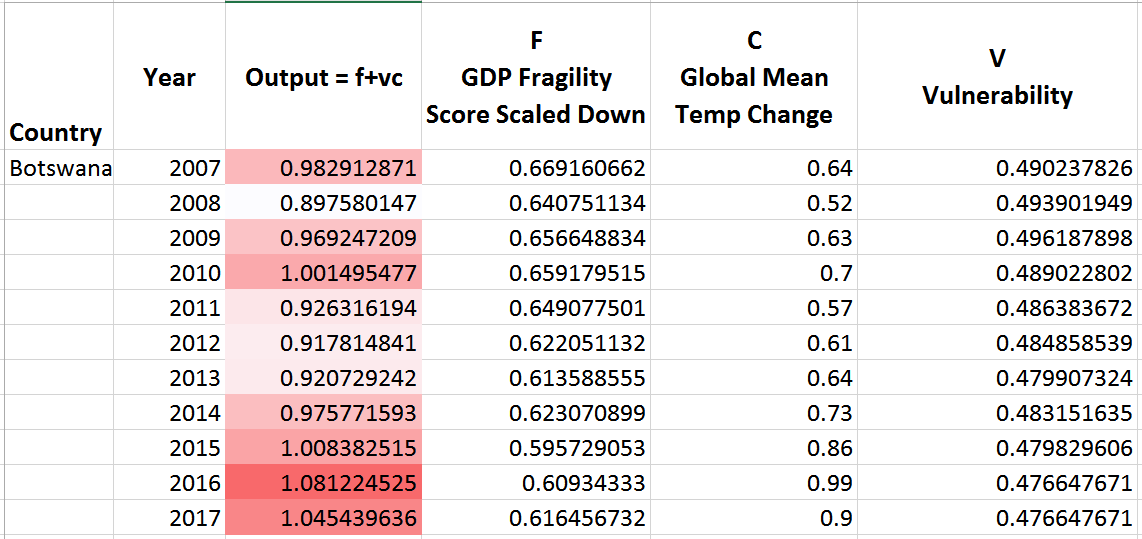
\includegraphics[scale=0.55]{Botswana_Model}
    \end{homeworkSection}
\end{homeworkProblem}
\newpage
\begin{homeworkProblem}[Task 2]
\begin{homeworkSection}
{Introduction}
In order to carry this out, several key observations regarding temperature fluctuations and GDP growth were made. Data gathered from the The World Factbook was vital to the overall assessment.
\end{homeworkSection}
\begin{homeworkSection}{Rational}
To carry out this task, the decision was made to choose Chad. The decision to use Chad was not an arbitrary one. Using the fact that rising temperatures due to climate change affects the agricultural output of certain fragile states, the top ten most fragile states were ranked based on agriculture as a percentage of their GDP. Based on this new ranking system, Chad was chosen due to agriculture accounting for 59 percent of their GDP (The World Factbook). After this, the Chad's GDP over all the years between 1980 to 2018 were analyzed in order to correlate temperature fluctuations due to climate change with their GDP over the same time period.
\end{homeworkSection}

\begin{homeworkSection}{Solution}
As stated above, temperature fluctuations from all the years between 1980 to 2018 were analyzed in order to produce the following graph:\\
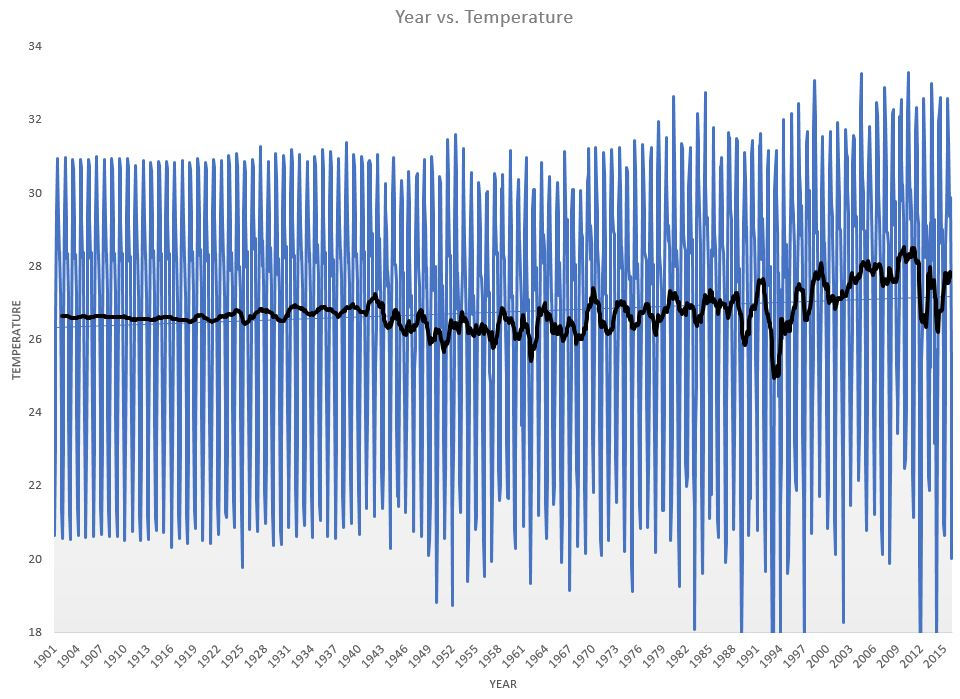
\includegraphics[width=16.5cm, height=10cm]{Capture3}\\
Based on this visual, it becomes patently obvious that Chad's overall surface temperature fluctuates more wildly as time progresses.
\newpage
The following graph represents the same data, but with a different visual in order to see the trend more clearly.\\
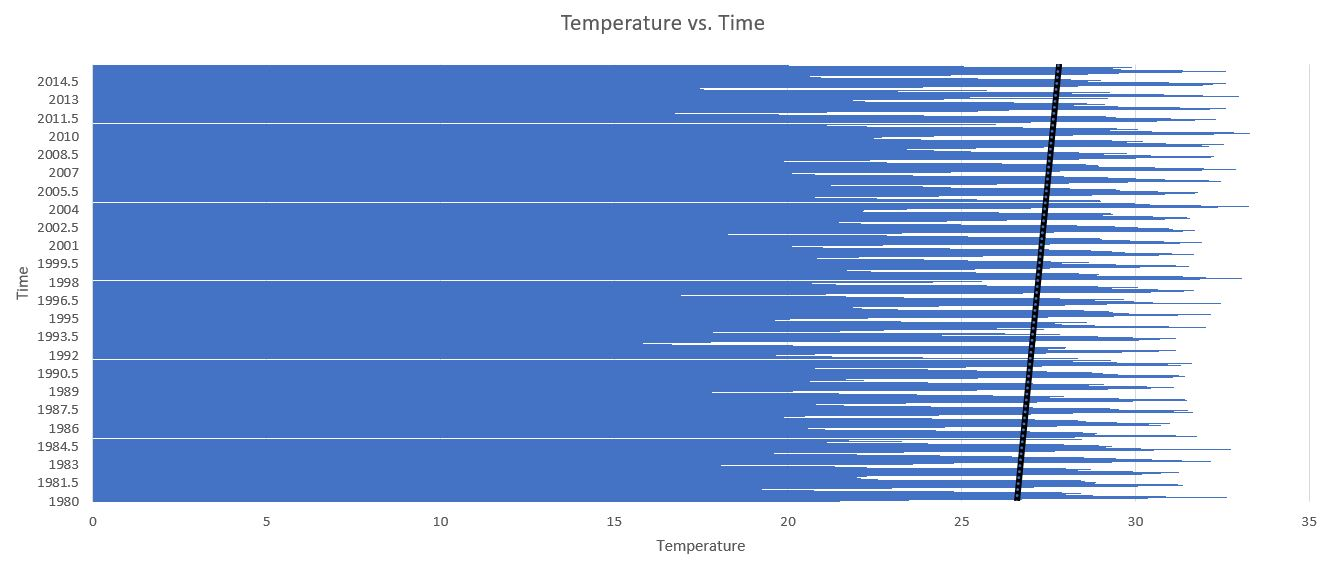
\includegraphics[width=16.5cm, height=9cm]{Capture4}\\
Now it becomes apparent that Chad's overall surface temperature is changing with an overall positive trend. Based on the two graphs shown above, it was determined that not only is the surface temperature of Chad fluctuating more wildly as time progresses, but these fluctuations are tending towards hotter overall temperatures.\\
\\
Data regarding Chad's growth in GDP was gathered from The International Monetary Fund and then analyzed. The data that was used focused on the years from 1980 to 2018. From this, the following graph was produced:


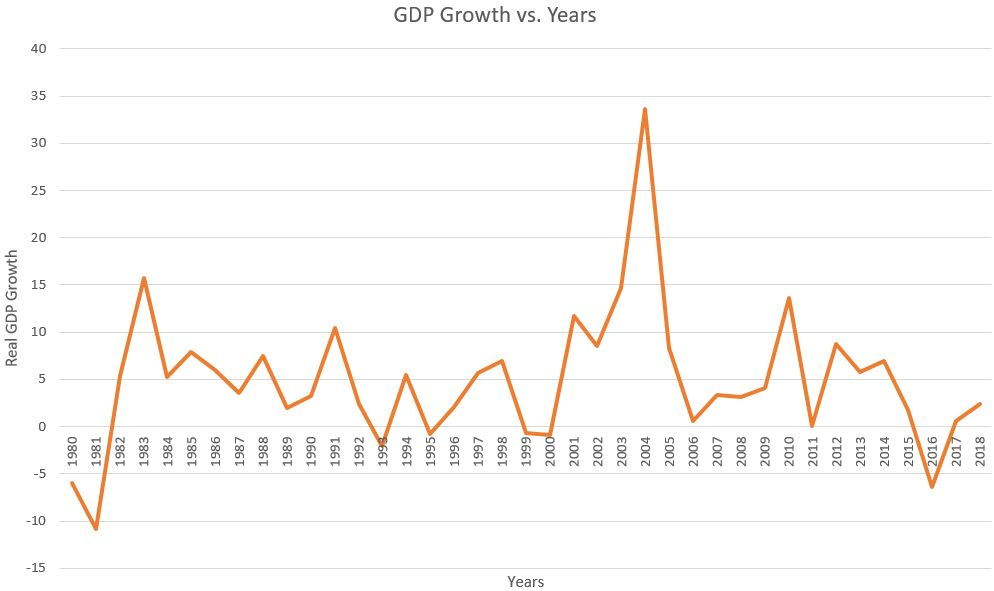
\includegraphics[width=16.5cm, height=8cm]{Capture5}\\
Based on this graphic there are clear fluctuations in Chad's GDP (as one would expect), however there are certain periods when their GDP takes a massive dive, most notably are the years 2004 (The Chadian coup d'état attempt) and 2016 (the warmest on record). \\\\
All the collected data regarding Chad's GDP growth and surface temperature fluctuations serves as fairly strong evidence that suggests that the effects of climate change played a vital role in the fragility of Chad.
Based on the model, Chad's fragility was determined to be $1.50813243622840$. \\\\
In order to assess Chad's fragility without the effects of climate change, the model effectively becomes $f-cv$ which gives $0.949672588$. This change is enough to change to move Chad from the fragile category well into the vulnerable category.

\end{homeworkSection}

\end{homeworkProblem}
\newpage
\begin{homeworkProblem}[Task 3]
    \begin{homeworkSection}{Introduction}
        Botswana is a nation in Sub-Saharan Africa, ranked $120^{th}$ on the FSI, with a score of $63.8$, just above half that of the top-ranked South Sudan. However, in the model created, Botswana is ranked $70^{th}$, the $10^{th}$ most fragile of all the nations in the Critical Zone.
    \end{homeworkSection}
    \begin{homeworkSection}{Rationale}
        The `tipping point' was considered to mean when a country `tips' from the Critical Zone into the bin of Fragile States. So a prediction of a country crossing this tipping point was simply a prediction over time, with the reference point being the tipping point. The tipping point also changes over time, but a constant one must be considered, so the average over recent years was used.
    \end{homeworkSection}
    \begin{homeworkSection}{Solution}
        A crucial definitive indicator of climate change induced fragility in Botswana deals with the increasing variability of rainfall. Climate change will intensify these already existing issues in that precipitation will decrease, but with an increased risk of flooding, droughts will increase, and groundwater recharge will decrease. These effects will then negatively impact Botswana's subsistence and commercial agricultural sectors, safe yields from dams, and tourism attractions such as the Okavango Delta.  These negative effects will increase Botswana’s overall fragility.\\\\
        The exact value at which a country is Fragile or not changes from year to year. The average, over 2017-2015 is $1.11597722889870$. This is the de-facto tipping point, which can be adjusted.\\
        To predict when Botswana may reach this tipping point uses the information of this model over the ten-year period for which reliable data exists. Linear, Polynomial Degree 3, and Polynomial Degree 6 trend-lines show some possible projections.\\
        The more general, although conservative, linear estimate predicts this will be within 10 years; whereas the polynomial regression predict that Botswana will be a Fragile State in the following year or two.\\
        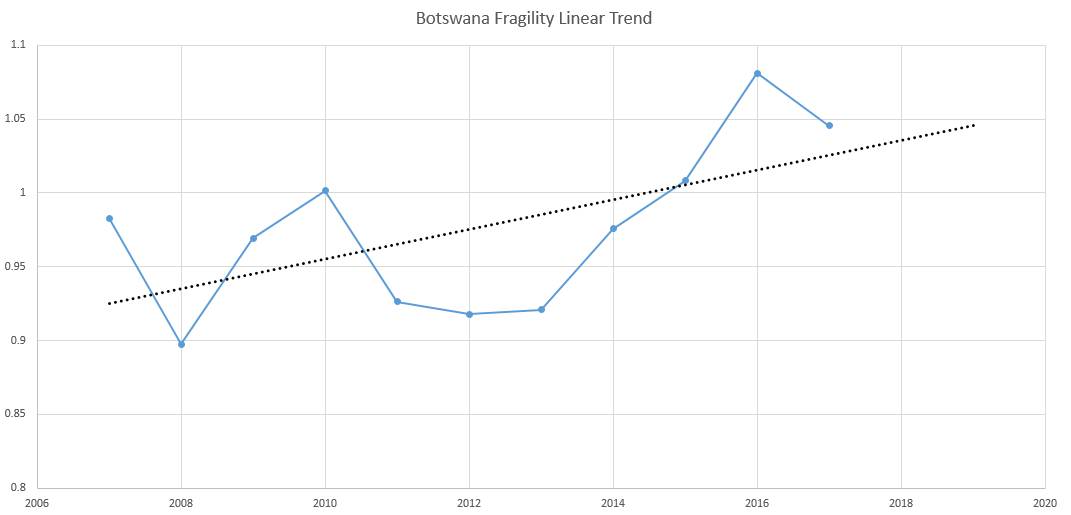
\includegraphics[scale=0.515]{Botswana_Linear}\\
        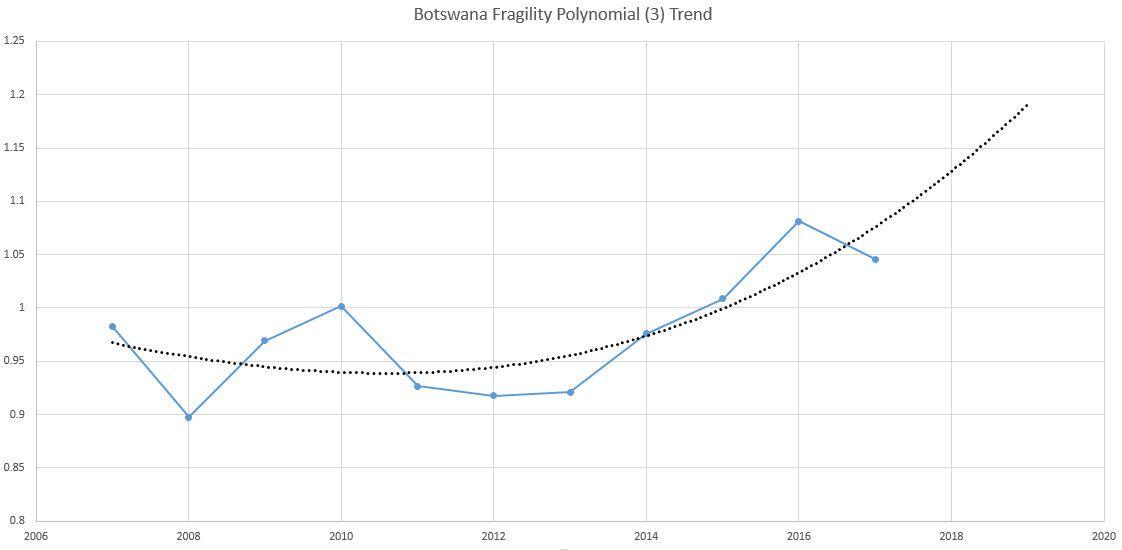
\includegraphics[scale=0.575]{Botswana_P3}\\
        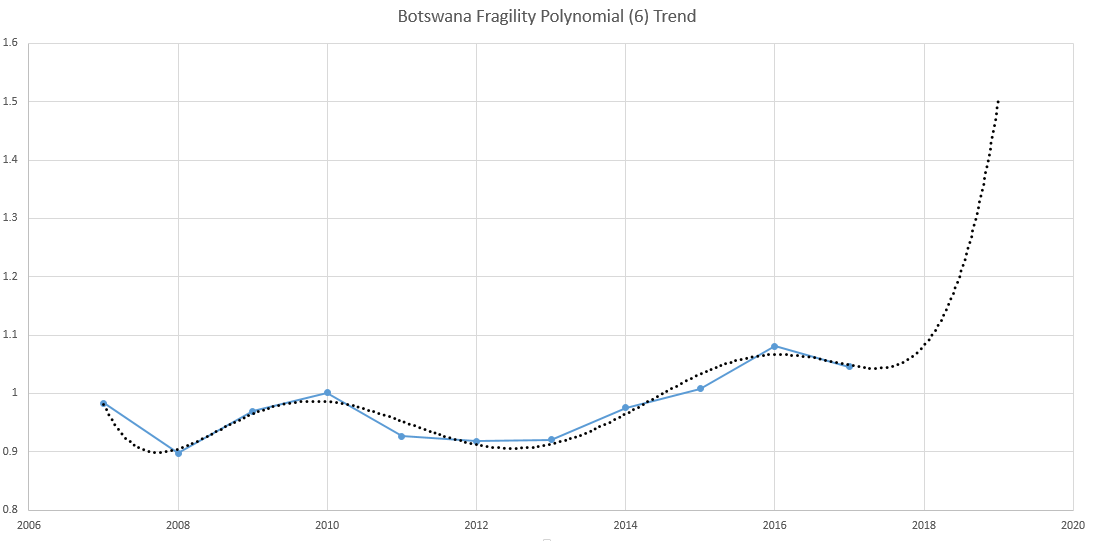
\includegraphics[scale=0.6]{Botswana_P6}
    \end{homeworkSection}
\end{homeworkProblem}
\newpage
\begin{homeworkProblem}[Task 4]
    \begin{homeworkSection}{Introduction}
        Countries are impacted by Climate Change in vastly different ways. Not only in amount, but type, for example inland countries would face droughts whereas coastal countries would face sudden natural catastrophic disasters. Furthermore, countries are differently equipped to deal with these issues. State driven interventions for particular nations are considered to be for the nation rather than for the prevention of Climate Change. Though it is noteworthy that any such `solution' is not sustainable; to treat a problem such as Climate Change, one treats the root, not the individual symptoms.
    \end{homeworkSection}
    \begin{homeworkSection}{Rationale}
        To consider every nation's weaknesses and cost of adjustment is (especially in the scope of this project) impossible. Instead, the developing nations in each Climate region were partitioned and considered.\\\\
        The components that determine vulnerability are as follows: food, water, health, ecosystem services, human habitat and infrastructure. These sectors were then narrowed down to what could be affected by government interventions: food, water, health, infrastructure (human habitats also deals with infrastructure). This shows that within this model, effective risk mitigating governmental intervention measures could include agricultural programs, clean water access programs, medical programs (that deal with Climate Change induced illnesses), and infrastructure programs.\\\\
        The proposed interventions are measured in terms of Millions of Dollars expenditure, as in the figure below. This is particularly useful because there are already expenditures in place, some of which may even need to be downsized, such as Irrigation Expansion.\\\\
        The effects of these investments are measured in terms of nutrition, which serves as a good metric; food and water are the most basic necessities, and the improvement of roads and irrigation also allow for basic hygiene and (if need be) evacuation.
    \end{homeworkSection}
    \begin{homeworkSection}{Methodology}
        Fortunately, Table 10 from \textit{Climate Change: Impact on Agriculture and Costs of Adaptation} outlines how additional investments should be distributed, by both region and sectors of improvement (that directly are, or consequently improve, the components above). This serves as a foundation for state-driven intervention. The average of the two scenarios was taken, and then also adjusted for inflation.\\\\
        Then, to make this meaningful for each country, using the model, a country's relative fragility is assessed, and used to distribute to each country. Relative fragility for a country was calculated by dividing its fragility score over the sum of all scores, with the idea in mind that any monetary solution would be distributed to all countries.
    \end{homeworkSection}
    \begin{homeworkSection}{Solution}
        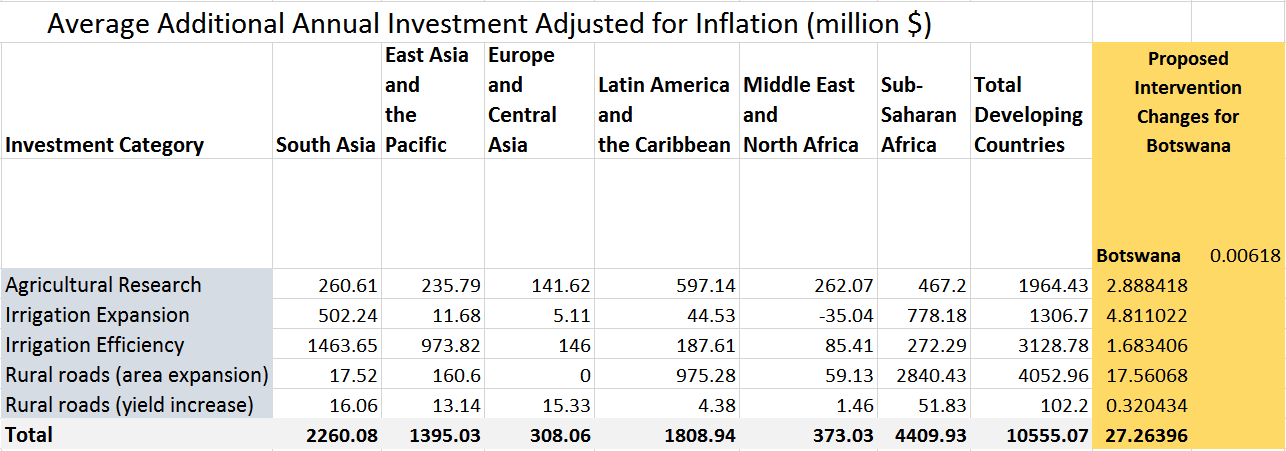
\includegraphics[scale=0.5]{Table10Botswana_Short}\\
        As an extending example, included in the table updated from Table 10, is the proposed intervention for Botswana. Reflective of it's Climate Change Fragility and it's case study: road and irrigation networks stand to improve significantly, aiding in resource supply efficiency and distribution of water to people and land, with a total investment change of just above $27M$ in current USD.
    \end{homeworkSection}
\end{homeworkProblem}
\newpage
\begin{homeworkProblem}[Task 5]
    This model would not be effective for smaller ``states” or larger ``states.”  This model is specifically dependent on information regarding characteristics of entire countries. The indicators that contribute to the baseline fragility factor, F, and the vulnerability to the effects of climate change factor, V, come from things like GDP, national security, public services, national resources, etc. In order to scale the model down to a city or up to a continent, the V and F components would require new, unique values depending on the areas being analyzed. The climate change factor, C,  will be the best adjustment to a smaller region, because the current C simply represents average global temperature change in the model; the local temperature change is much more indicative of its effect on certain aspects of Climate Change, like drought. The global temperature change should still be taken into account for non-local effects, such as natural disasters that take form far from a country before it devastates one.\\\\
    Scaling up to a continent could be done by combining the V and F values for all the countries within the given continent. However, additional factors may also need to be considered. For example, within the F value,  the indicator “group grievance” may need to be reconsidered in particularly volatile regions where there are more historical tensions between neighboring nations.\\\\
    Scaling down to a city would take considerably more new data to determine the new F and V values. Information for a given city could be much more refined and specific, but that unique data would need to be acquired for the given area being analyzed. Based on the set up of this model, cities may need to be analyzed case by case. The general country-wide data used was found through commonly conducted research. Research for a particular city may need to be specifically conducted and organized in order to assign any given city with its own F and V values.
\end{homeworkProblem}
\newpage

\begin{homeworkProblem}[Works Cited]
    \textit{Botswana Environmental and Climate Change Analysis} . 2008, pp. 1–21, \textit{Botswana Environmental and Climate Change Analysis} .\\\\
    ``2004 Chadian Coup D`état Attempt.'' \textit{Wikipedia}, Wikimedia Foundation, 12 Feb. 2018,\\ en.wikipedia.org/wiki/2004\_Chadian\_coup\_d\%27\%C3\%A9tat\_attempt.\\\\
    Chen, C., et al. ``University of Notre Dame Global Adaptation Index.'' \textit{Notre Dame Global Adaptation Initiative}, University of Notre Dame, 2018, gain.nd.edu/our-work/country-index/.\\\\
    Glick, Daniel. ``GeoSigns: The Big Thaw .'' \textit{National Geographic}, Sept. 2004,\\ ngm.nationalgeographic.com/ngm/0409/feature2/fulltext.html.\\\\
    ``Global Data.'' \textit{Fragile States Index}, The Fund for Peace, 2017, fundforpeace.org/fsi/.\\\\
    Index Mundi. ``GDP - per Capita (PPP).'' 2017.\\\\
    International Monetary Fund. ``Real GDP Growth: Annual Percent Change, Chad.'' 2017.\\\\
    The World Bank Group. ``Climate Change Knowledge Portal, Chad, Temperature.'' 2018.\\\\
    The World Bank Group. ``GDP Per Capita(Current U.S.\$), All Countries and Economies.'' 2018.\\\\
    Nelson, Gerald C., et al. \textit{Climate Change: Impact on Agriculture and Costs of Adaptation}. International Food Policy Research Institute, 2009.\\\\
    NASA/GISS. ``The Change in Global Surface Temperature Relative to 1951-1980 Average Temperatures.''\\\\
    United States, Congress, US Bureau of Labor Statistics . ``Consumer Price Index(CPI) Inflation Calculator .'' \textit{Consumer Price Index(CPI) Inflation Calculator} .\\\\
    ``What's in a Name? Weather, Global Warming and Climate Change.'' NASA, NASA, 19 Jan. 2016, climate.nasa.gov/resources/global-warming/.
\end{homeworkProblem}
\end{spacing}
\end{document}

%%%%%%%%%%%%%%%%%%%%%%%%%%%%%%%%%%%%%%%%%%%%%%%%%%%%%%%%%%%%%

%----------------------------------------------------------------------%
% The following is copyright and licensing information for
% redistribution of this LaTeX source code; it also includes a liability
% statement. If this source code is not being redistributed to others,
% it may be omitted. It has no effect on the function of the above code.
%----------------------------------------------------------------------%
% Copyright (c) 2007, 2008, 2009, 2010, 2011 by Theodore P. Pavlic
%
% Unless otherwise expressly stated, this work is licensed under the
% Creative Commons Attribution-Noncommercial 3.0 United States License. To
% view a copy of this license, visit
% http://creativecommons.org/licenses/by-nc/3.0/us/ or send a letter to
% Creative Commons, 171 Second Street, Suite 300, San Francisco,
% California, 94105, USA.
%
% THE SOFTWARE IS PROVIDED "AS IS", WITHOUT WARRANTY OF ANY KIND, EXPRESS
% OR IMPLIED, INCLUDING BUT NOT LIMITED TO THE WARRANTIES OF
% MERCHANTABILITY, FITNESS FOR A PARTICULAR PURPOSE AND NONINFRINGEMENT.
% IN NO EVENT SHALL THE AUTHORS OR COPYRIGHT HOLDERS BE LIABLE FOR ANY
% CLAIM, DAMAGES OR OTHER LIABILITY, WHETHER IN AN ACTION OF CONTRACT,
% TORT OR OTHERWISE, ARISING FROM, OUT OF OR IN CONNECTION WITH THE
% SOFTWARE OR THE USE OR OTHER DEALINGS IN THE SOFTWARE.
%----------------------------------------------------------------------%
